\chapter{Introduction to OS Security}

Linux, as well as other OSs, uses variety of methods to protect the system and the data. The chapters in this part of the notebook introduce some of these security methods. As cloud computing is getting more and more popular, virtualization security is also discussed.

\section{Basics}

The background, motivation, and basic concepts of computer security are introduced in this section.

\subsection{Risks and Attacks}

No computer or OS are absolutely safe. Risks can be introduced by the subjects listed below.
\begin{itemize}
	\item Software bugs. The OS and application software may have bugs which leave backdoors to malware.
	\item Malicious users. A user may perform illegal actions that damage other users sharing the same servers or services.
	\item Unauthorized access. The user or a program may intentionally or accidentally try to access confidential data that they should not view.
\end{itemize}
A risk will most likely not turn into an actual disaster by nature. However, when a hacker or a malicious user initiate an attack deliberately taking advantage of the risk, it may cause troubles.

The attacks can be divided into the following categories.
\begin{itemize}
	\item Malware. The attacker disguises a piece of malware code as a legitimate software. When the software is executed, the malware carries out harmful activities.
	\item System Penetration. The attacker accesses a protected system bypassing security checks.
	\item Man-in-the-Middle Attack (MitM). The attacker intercepts communications between legitimate entities, and steal or modify the contents of the communication.
	\item Denial of Service (DoS). The attacker overwhelms a system and paralyzes its service by sending a lot of requests to the system, more than it can handle.
	\item Network Sniffing. The attacker passively logs information from the internet, and use them for future attacks.
	\item TEMPEST (Van Eck phreaking). The attacker collects and analyses data measured from electromagnetic emissions of devices such as mobile phones, and decode information from the measurements.
	\item Social Engineering. The attacker gathers information of the victims by cheating, phishing emails, etc.
\end{itemize}

To protect the users from the attacks, we need both computer security and communication security. This notebook focuses on computer security, specifically OS security.

\subsection{General Security Architecture}

It is impractical to secure every component of a system (hardware, OS kernel, OS services, application services, user interface, users, etc.) with a singular universal protection method. Therefore, a more common approach is to implement a layered security architecture as shown in Fig. \ref{ch:ossec:fig:layerstructure}. In this paradigm, the system is segregated into distinct layers such as the hardware layer, the OS layer, and the application layer. Each layer employs its own security mechanisms targeting specific vulnerabilities.
\begin{figure}[htbp]
	\centering
	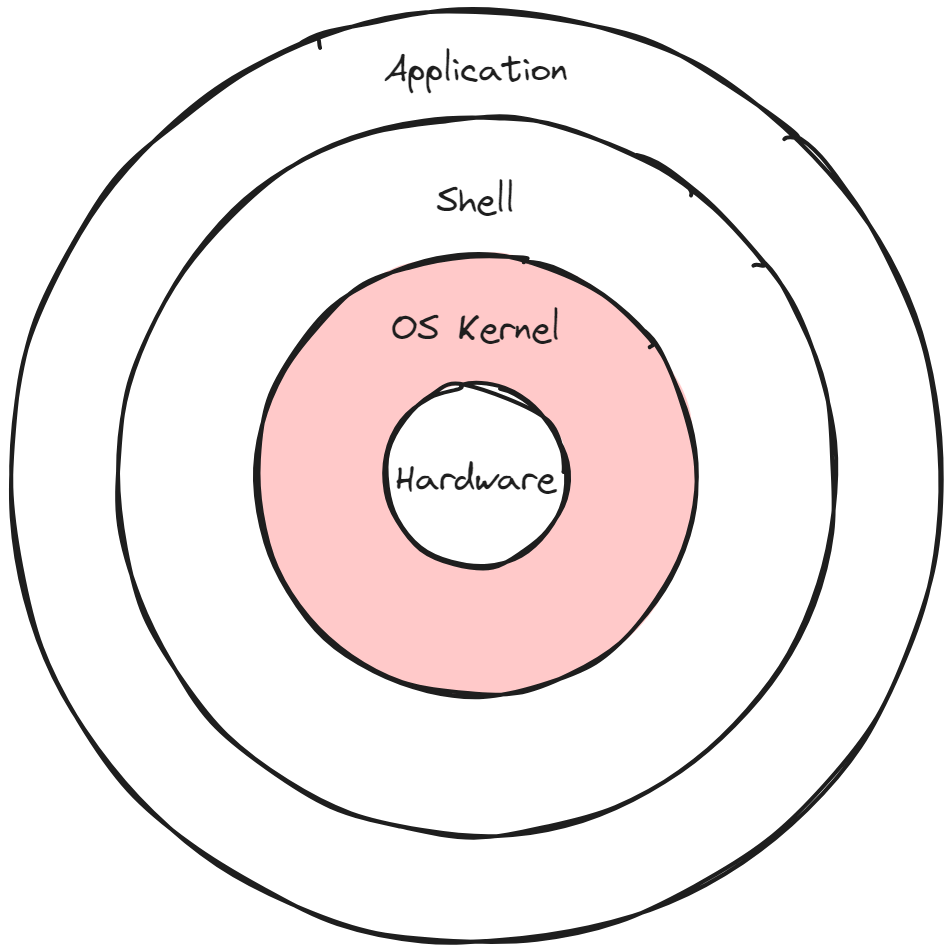
\includegraphics[width=200pt]{chapters/part-4/figures/os_layer.png}
	\caption{Layer structure of an operating system.} \label{ch:ossec:fig:layerstructure}
\end{figure}

Among all these layers, securing the OS is particularly crucial for several reasons:
\begin{itemize}
	\item Breaches in both hardware and application software often exploit vulnerabilities within the OS. By securing the OS, threats to other layers can be substantially mitigated. Even if certain applications are compromised, a robust OS can limit the extent and spread of the damage.
	\item If the OS is compromised, safeguarding other layers becomes extremely difficult. Most components across layers interact frequently with the OS and they typically operate under the assumption that the OS is trustworthy.
\end{itemize}

A system is considered secure if the following criteria are met.
\begin{itemize}
	\item It is secure upon booting, and
	\item It never perform an action so that it can become insecure from a secure condition.
\end{itemize}
Notice that just for clarification, there are some slight differences between ``secure'' and ``trusted'' as follows. System security is the ultimate goal. A system is either secure or insecure, and we want it to stay secure all the time. Trustworthy, on the other hand, is a graded feature that we use to describe an entity in the system. We can, for example, say which parts (services, users, etc.) of the system is trustworthy, and to what extent they can be trusted.

\subsection{Standards and Requirements}

There are many official standards on computer security. For example, Trusted Computer System Evaluation Criteria (TCSEC) published in 1985, also known as the ``orange book'', is one of the earliest standards in this domain. It divides system into different tiers in terms of security, including
\begin{itemize}
	\item A: Verified protection
	\item B: Mandatory protection
	\begin{itemize}
		\item B3: Security Domains
		\item B2: Structured Protection
		\item B1: Labeled Security Protection
	\end{itemize}
	\item C: Discretionary protection
	\begin{itemize}
		\item C2: Controlled Access Protection
		\item C1: Discretionary Security Protection
	\end{itemize}
	\item D: Minimal protection
\end{itemize}
Notice that TCSEC is considered outdated due to the rapid advancement of technology. Nowadays, commercialized PCs and OS such as Windows 11 pro, MacOS, RHEL, implement robust security mechanisms that align with various aspects of TCSEC criteria of different tiers, some of which required by Tier B and even Tier A. While TCSEC remains a classic and milestone, newer standards have been developed and adopted globally by various countries and organizations.

In the scope of Linux, there is an open-project, ``Security Enhanced Linux (SELinux)'' that enables mandatory access control in Linux. It started as an add-on module of Linux kernel, and today it has become a default module.

In general, the requirements of secure computer systems include
\begin{itemize}
	\item Confidentiality. Data, as well as the existence of the data, is not leaked to unauthorized entities.
	\item Integrity. The data can be trusted, and it cannot be modified by unauthorized entities.
	\item Accountability. It is possible to trace and audit the actions performed by users and programs.
	\item Availability. The system should be resistant to attacks and consistently provide services.
\end{itemize}
The primary objective of studying computer security is to ensure that the aforementioned requirements are consistently met and upheld. Regrettably, there is no systematic approach guaranteeing that these requirements are met at all times.

\section{Elements of Security}

Key components in security schema include:
\begin{itemize}
	\item Security policy. It defines what needs to be protected and what the desired security outcomes are.
	\item Security mechanism. It defines the tools, methods, and procedures employed to enforce the security policy.
	\item Security assurance: It defines the means by which we evaluate the efficacy of the security mechanism.
\end{itemize}

\subsection{Security Policy}

A security policy establishes the standards and objectives that a system must adhere to, outlining the rules that both users and programs are expected to follow. Deviations from these stipulations or breaches of the rules can compromise the security of the system. A security policy often comprises a set of sub-policies, which may be categorized into areas like confidentiality policies, integrity policies, and so on.

Different systems may implement different policies. There are two commonly seen security policies that concern most of the systems. They are
\begin{itemize}
  \item Confidentiality policies: preventing the unauthorized disclosure of information.
  \item Integrity policies: preventing the unauthorized alteration of information.
\end{itemize}

For the sake of clarity and to ensure that no misunderstandings arise, it is crucial for the security policy to be articulated in a precise and consistent manner. Instead of relying on colloquial or vague terminology, we use security policy model and policy language to formally and precisely describe the security policy. Security policy model should be ambiguity-free and easy to comprehend. Though it does not assume or restrict the security mechanism to be used to fulfill the policy, it should give some guidance to how the mechanisms can be designed. At the minimum, it should make sure that the policy is reachable.

More details of security policy, especially security model, is introduced in later sections. There are classic security models such as HRU model that has been proved useful and inspiring.

\subsection{Security Mechanism}

Security mechanisms are the means and tools to fulfill the security policies. Security mechanisms can be widely divided into 3 types:
\begin{itemize}
  \item Prevention: (most commonly seen) protect system from being damaged.
  \item Detection: detect potential risks and damages.
  \item Recovery: recover a compromised system back to a secure system.
\end{itemize}

Different systems uses different security mechanisms to fulfill different security policies. Some important concepts are introduced below.

One of the most commonly used security mechanisms is access control, which monitors and controls the accessibility of a resource (known as objects) from users or programs (known as subjects). Access control is managed by reference monitor. Reference monitor refers to the combination of hardware and software that practices access control using the architecture given in Fig. \ref{ch:ossec:fig:reference_monitor}.

\begin{figure}[htbp]
	\centering
	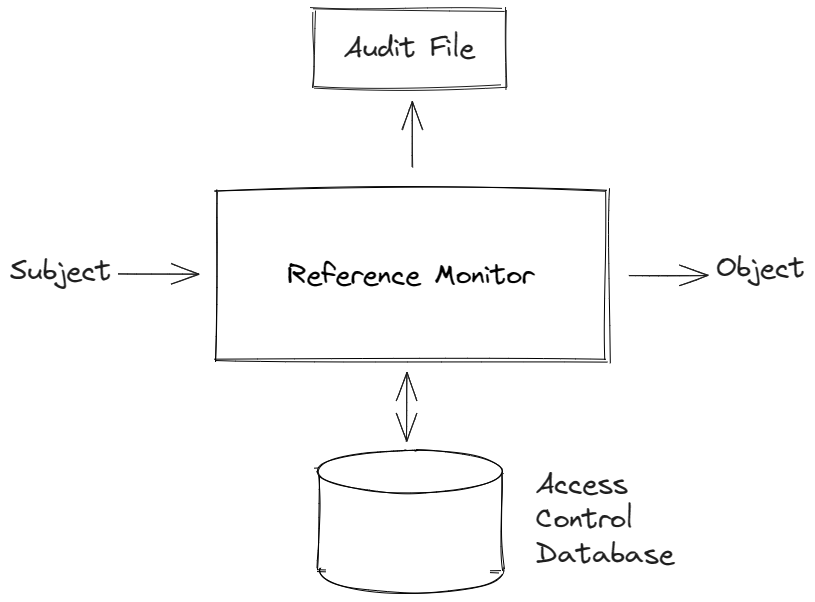
\includegraphics[width=200pt]{chapters/part-4/figures/reference_monitor.png}
	\caption{Reference Monitor Architecture.} \label{ch:ossec:fig:reference_monitor}
\end{figure}

Another important concept is security kernel. Security kernel refers to a small piece of code running in the kernel of OS that addresses system security.

Both reference monitor and security kernel shall have the following features:
\begin{itemize}
  \item Completeness. They must be active all the time, and no process can bypass them.
  \item Isolation. Their content cannot be modified by unauthorized personals.
  \item Verification. They can be audited, and their effectiveness can be proved and verified. (This implies that their realization cannot be too complicated.)
\end{itemize}

\subsection{Security Assurance}

Security assurance refers to the degree of confidence in the security features, practices, procedures, and architecture of an information system. It ensures that the system enforces the security policy effectively. Below are key aspects of security assurance:

\begin{itemize}
	\item \textbf{Verification and Validation}:
	\begin{itemize}
		\item Verification: Checking that the system complies with specifications and is correctly implemented.
		\item Validation: Ensuring the system meets user's needs and its intended purpose.
	\end{itemize}
	
	\item \textbf{Assessment and Evaluation}:
	\begin{itemize}
		\item Evaluating the effectiveness of security controls.
		\item Assessing compliance with security standards.
	\end{itemize}
	
	\item \textbf{Testing}:
	\begin{itemize}
		\item Conducting tests to identify security vulnerabilities.
		\item Penetration testing and automated vulnerability scanning.
	\end{itemize}
	
	\item \textbf{Certification and Accreditation}:
	\begin{itemize}
		\item Certification: Evaluation of security features of a system.
		\item Accreditation: Approval to operate in a secure environment.
	\end{itemize}
	
	\item \textbf{Risk Management}:
	\begin{itemize}
		\item Identifying, assessing, and mitigating risks.
	\end{itemize}
	
	\item \textbf{Audit and Compliance}:
	\begin{itemize}
		\item Regular audits for policy and standard compliance.
		\item Maintaining logs and records for security events.
	\end{itemize}
	
	\item \textbf{Continuous Monitoring}:
	\begin{itemize}
		\item Real-time threat detection and response.
	\end{itemize}
	
	\item \textbf{Documentation}:
	\begin{itemize}
		\item Maintaining records of security policies, procedures, and changes.
	\end{itemize}
	
	\item \textbf{Training and Awareness}:
	\begin{itemize}
		\item Training users and administrators in security best practices.
		\item Creating organizational awareness of security threats.
	\end{itemize}
\end{itemize}

Security assurance is an ongoing process that is critical for ensuring that a system is secure by design, in implementation, and in deployment, adapting to new vulnerabilities and attack vectors over time.

\subsection{Trusted Computing Base}

System boundary refers to the boundary between the system and outside world. Everything in the system is protected by the system following the requirements specified by the security policy. 

Security perimeter refers to the imaginary boundary that distinguishes security-relevant components and non-security-relevant components in the system. Security-relevant components include OS, system files, administrators and his files and programs, etc. Non-security-relevant components include user program, user profiles, I/O devices, etc. A demonstrative figure from \cite{gasser1988building} is given in Fig. \ref{ch:ossec:fig:system_boundary}. 

\begin{figure}[htbp]
	\centering
	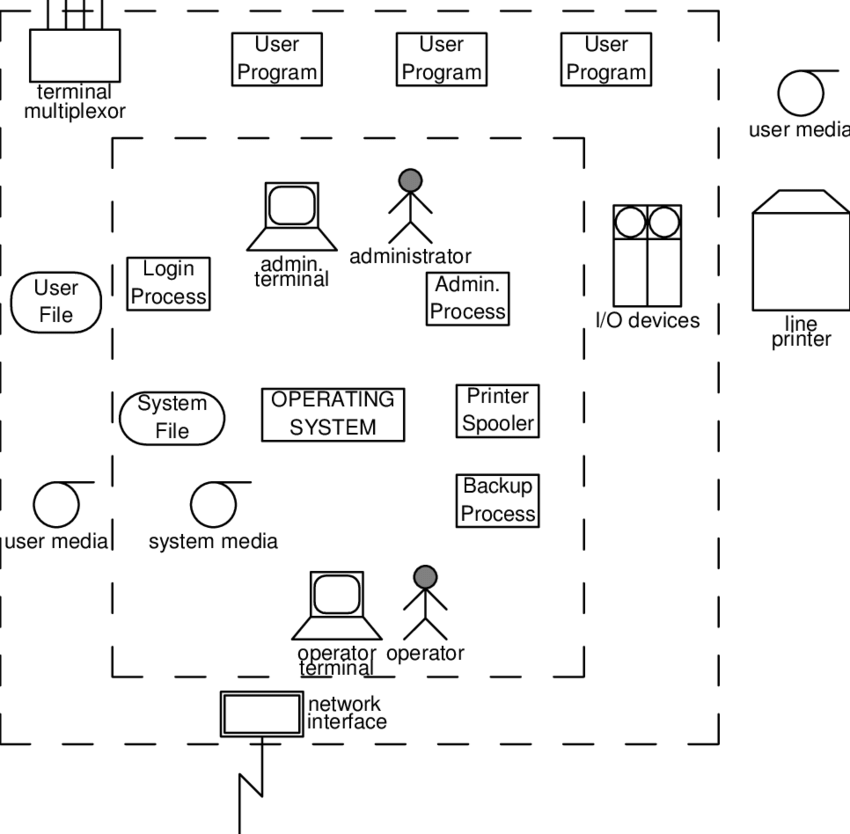
\includegraphics[width=300pt]{chapters/part-4/figures/system_boundary.png}
	\caption{Reference Monitor Architecture \cite{gasser1988building}.} \label{ch:ossec:fig:system_boundary}
\end{figure}

The Trusted Computing Base (TCB) encompasses all the hardware and software components that are crucial for enforcing a system's security policy. This dual perspective implies that:

\begin{itemize}
	\item Security Assurance. Efforts must be made to ensure that the TCB components are as secure as possible. Any vulnerability within the TCB could potentially compromise the security of the entire system. Therefore, the integrity, confidentiality, and availability of the TCB are of utmost importance.
	\item Assumption of Trust. When designing security mechanisms for the system, the TCB is assumed to be inherently secure and trustworthy. Security mechanisms rely on the TCB to operate correctly and to enforce security policies effectively. This assumption is fundamental to the system's architecture, as the TCB underpins the security of all other components.
\end{itemize}

The TCB can be likened to a police department in a city. Just as citizens rely on the police force to uphold the law and protect public safety, a system relies on the TCB, the ``police security bureau'' of the system, to enforce its security policies and maintain the integrity of its operations. Similarly, the well-being and readiness of the police officers are paramount to the security of the city. In the case of the TCB, ensuring the security of these trusted components is crucial because a compromise to any part of the TCB could undermine the security of the entire system. The system defenses are only as robust as the TCB's integrity and resilience.

Non-trusted components, while not central to the system security architecture, are analogous to the various elements of a city that the police department does not directly oversee. If these elements are compromised, the immediate risk is localized. However, securing non-trusted components is also important. We always want each and every component in the system to work properly. Maybe more importantly, we want to prevent them from becoming weak links that could be exploited to attack the TCB.

The goal is to keep the TCB, our ``police department'', as streamlined and strong as possible. A smaller, well-protected TCB simplifies the task of maintaining system security and reduces the potential attack surface.

\section{Access Control}

In the realm of computer security, a ``subject'' refers to an active entity that initiates an action, typically a user who takes an active role. On the other hand, an ``object'' refers to a passive entity that receives or is acted upon by the action. In most contexts, objects are files, data, or programs. Processes and threads can simultaneously act as both subjects and objects.

The term ``access'' is used to describe when a subject performs actions on an object. This can encompass various activities such as creating, reading, executing, editing, or deleting the object. Access control is a mechanism that assists systems in determining whether to grant or deny specific permissions, dictating which subjects can access particular objects and what actions they can undertake with those objects. 

Typically, a user who plays subject is required to first identify himself by logging into an account of the system using a valid authentication methods. A user or a program that plays subject needs to be assigned with a ``role''. The program can only execute if its role possesses the necessary permissions to do so, including access to required resources like CPU, memory, disk space, and databases.

We use access control matrix to describe the association of subject and object. A demonstrative graph is given in Fig. \ref{ch:ossec:fig:acmatrix}. In this demonstration, like introduced in Section \ref{ch:fm:sec:accesscontrollist}, ``read'', ``write'' and ``execute'' permissions are controlled, each using $3$-bit ``r'', ``w'' and ``x'', together forming the nine permission bits.
\begin{figure}[htbp]
	\centering
	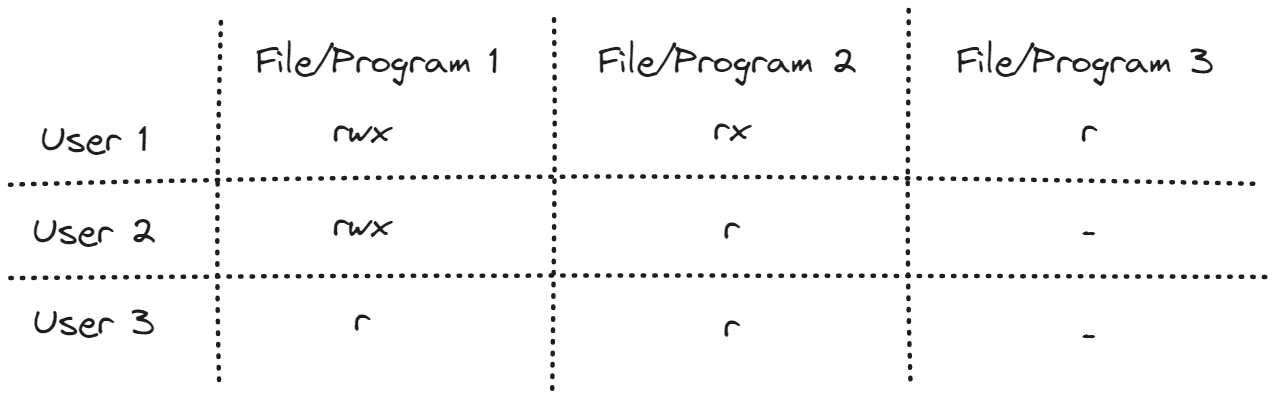
\includegraphics[width=300pt]{chapters/part-4/figures/acmatrix.png}
	\caption{A demonstration of access control matrix.} \label{ch:ossec:fig:acmatrix}
\end{figure}

The most popular ways to manage the access control matrix include discretionary access control (DAC) and mandatory access control (MAC).

\subsection{Discretionary Access Control}

In the DAC model, the owner of the data, or the group to which the owner belongs, determines the access control matrix for the data. This means that the owner has complete authority over who can access the data and in what manner. Additionally, the owner has the flexibility to delegate full access privileges to others if desired. This level of flexibility makes DAC a popular choice in many operating systems, including Linux.

Under DAC, the operating system can track the capability of each user's access to data. One method involves using a capability list, which outlines all the data a user can access. The users cannot modify their own capability lists. However, they can extend their access capabilities to other users. When a capability list is associated with each subject rather than individual users, it is referred to as a profile. Conversely, an object can be assigned an ACL as introduced in Section \ref{ch:fm:sec:accesscontrollist} that records which users or subjects have access. This latter method of assigning ACLs to objects is more widely adopted.

As mentioned in Section \ref{ch:fm:sec:accesscontrollist}, in Linux access control is managed through a system of ``9 permission bits''. These bits define the accessibility for three distinct user categories: the owner, the group (the primary group of the owner, or a group the owner specifies), and others. Each category's permissions are represented by three bits, indicating whether the data is readable (\verb|r| or \verb|-|), writable (\verb|w| or \verb|-|) and executable (\verb|x| or \verb|-|). 

While this method is straightforward, it does have limitations, notably its simplistic division of subjects into only three categories, which may not offer sufficient flexibility for all use cases. But it suits most of our needs on a personal computer.

\subsection{Mandatory Access Control}

Though flexible, DAC adds risks to the system. A malware such as a Trojan horse is able to change ACL of files on behalf of the data owner without his notice or permission. To tackle this issue, consider MAC instead. MAC is popular on machines with sensitive data, such as government servers.

Unlike DAC where the owner can change the ACLs of his files, when MAC is implemented, the owner cannot change the ACLs of the files. Only the system can change the ACLs of the files according to predefined security policies.

As a special case of mandatory access control, consider multi-label security mechanism. In this implementation, security labels are assigned to both subjects and objects. Only the subject with a equal or higher security level than the object can access that object.










